\chapter{Architectuurontwerp}
\label{chap:architectuur}

% \section{Ontwerpdoelen}
% \label{sec:ontwerpdoelen}

% Het architectuurontwerp van de voorgestelde oplossing vertrekt vanuit de vereisten en knelpunten die in hoofdstuk~\ref{chap:probleemanalyse} werden geïdentificeerd. Het doel is een architectuur uit te werken die natuurlijke vragen kan vertalen naar gecontroleerde zoekopdrachten over meerdere bedrijfsystemen heen.


% Een eerste ontwerpdoel is het ondersteunen van zoekopdrachten over meerdere databronnen. De architectuur moet kunnen omgaan met systemen die verschillen in \glspl{API}, authenticatiemechanismen en datamodellen, zonder dat deze complexiteit zichtbaar wordt voor de eindgebruiker.

% Een tweede ontwerpdoel is modulariteit. Door de architectuur op te delen in afzonderlijke componenten en gespecialiseerde agents wordt de interne structuur van het systeem overzichtelijker en beter onderhoudbaar.

% Daarnaast moet de architectuur ook uitbreidbaar zijn. Nieuwe databronnen moeten later kunnen worden toegevoegd zonder fundamentele wijzigingen aan de bestaande componenten. Ook moet de architectuur voorzien in een duidelijke scheiding van verantwoordelijkheden. Query-interpretatie, coördinatie, toegang tot databronnen en generatie van antwoorden mogen niet in één grote monolith samenvallen.

% Verder moet de oplossing veilige toegang tot bedrijfsdata ondersteunen. De architectuur moet bestaande authenticatie- en autorisatieregels respecteren en mag geen toegang verlenen tot informatie waarvoor een gebruiker in het bronsysteem geen rechten heeft.

% Een bijkomend doel is betrouwbaarheid. De architectuur moet niet uitsluitend steunen op generatieve output van een taalmodel, maar op effectief opgehaalde gegevens uit de gekoppelde systemen.

\section{Overzicht van de voorgestelde architectuur}
\label{sec:architectuur-overzicht}

Om aan deze ontwerpdoelen te voldoen werd gekozen voor een multi-agentarchitectuur met een centrale orchestrator en meerdere gespecialiseerde subagents. Deze orchestrator vormt het centrale coördinatiepunt van het systeem. Hij ontvangt de gebruikersquery, interpreteert de vraag, bepaalt welke agent of combinatie van agents relevant is.

Voor elke geïntegreerde databron wordt een afzonderlijke agent voorzien. In het prototype gaat het om een Microsoft Graph agent, een Salesforce-Agent en een SmartSales-Agent. Elke agent bundelt de logica die nodig is om met één specifiek systeem te communiceren, inclusief kennis over de relevante \glspl{API}, querymogelijkheden, authenticatie en systeem-specifieke datamodellen.

De communicatie tussen agents en databronnen verloopt via een \gls{MCP}-gebaseerde integratielaag. Dit maakt het mogelijk om de agentlogica en de externe systemen los te koppelen, wat de onderhoudbaarheid en uitbreidbaarheid van het systeem vergemakkelijkt.

Het globale systeem kan worden opgevat als een gelaagde architectuur. Bovenaan bevindt zich de gebruikersinteractie via natuurlijke taal. Daaronder bevindt zich de orchestrator, die instaat voor interpretatie en coördinatie. Vervolgens zijn er de gespecialiseerde agents, die elk via \gls{MCP} en onderliggende \gls{API}-koppelingen communiceren met hun respectieve databronnen. De opgehaalde resultaten worden teruggestuurd naar de orchestrator, die deze samenbrengt en omzet in een bruikbaar antwoord voor de gebruiker. Figuur~\ref{fig:architectuur-overzicht} geeft een schematisch overzicht van deze architectuur.

\begin{figure}[htbp]
    \centering
    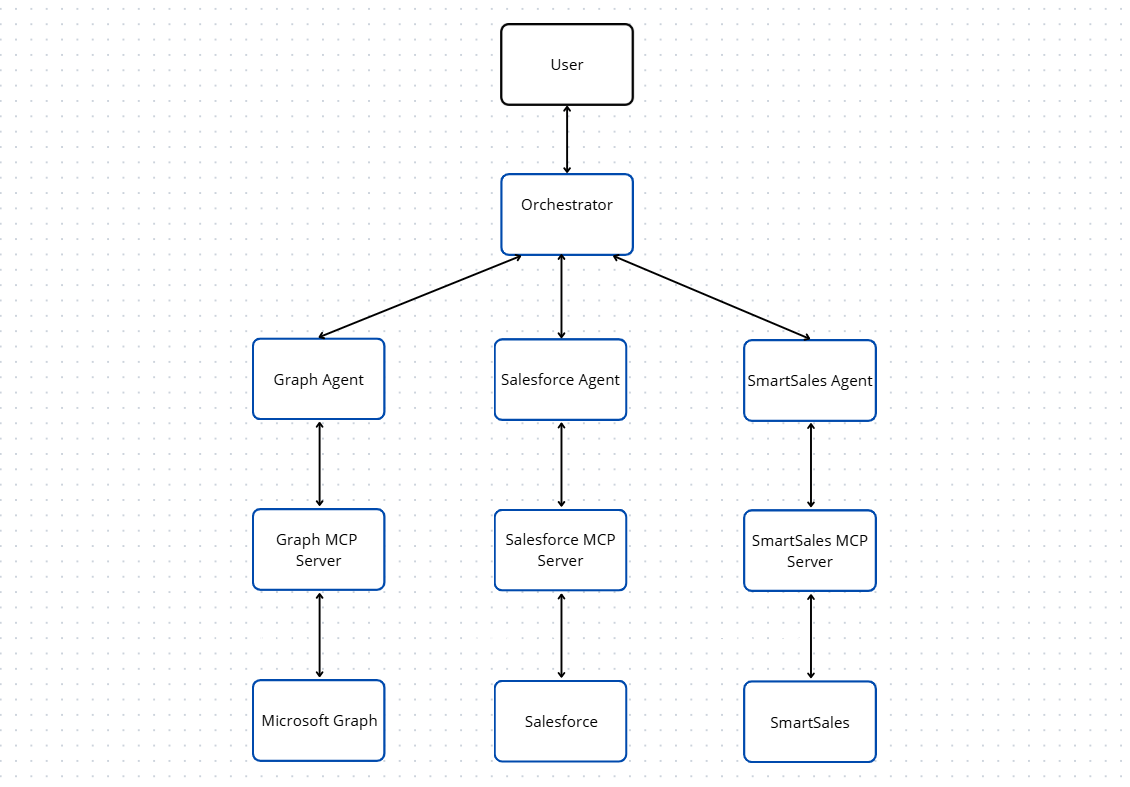
\includegraphics[width=0.80\textwidth]{diagram}
    \caption{Overzicht van de voorgestelde multi-agentarchitectuur: de orchestrator coördineert drie gespecialiseerde subagents (Graph Agent, Salesforce-Agent en SmartSales-Agent), die elk via een afzonderlijke MCP-server communiceren met hun onderliggende databron.}
    \label{fig:architectuur-overzicht}
\end{figure}

\section{Beschrijving van de componenten}
\label{sec:componenten}

\subsection{Orchestrator}
\label{subsec:orchestrator}

De orchestrator vormt het centrale coördinatiepunt van de voorgestelde architectuur. Hij ontvangt de natuurlijke taalquery van de gebruiker en stuurt het verdere zoekproces aan.

De orchestrator interpreteert de gebruikersvraag en bepaalt welke gespecialiseerde agent of combinatie van agents nodig is om deze te beantwoorden. Bij eenvoudige zoekopdrachten volstaat één agent, terwijl bij complexere vragen meerdere agents na elkaar of in combinatie kunnen worden aangesproken.

Daarnaast verzamelt de orchestrator de resultaten van de betrokken agents en brengt hij deze samen tot één antwoord dat aansluit bij de oorspronkelijke vraag van de gebruiker. De orchestrator is dus verantwoordelijk voor query-interpretatie, routing, coördinatie en antwoordsynthese, maar bevat zelf geen systeem-specifieke integratielogica.

\subsection{Gespecialiseerde agents}
\label{subsec:gespecialiseerde-agents}

Voor elke geïntegreerde databron wordt een afzonderlijke gespecialiseerde agent voorzien. In het prototype gaat het om een Microsoft Graph-Agent, een Salesforce-Agent en een SmartSales-Agent.

Deze opsplitsing is nodig omdat de betrokken systemen sterk verschillen in \glspl{API}, authenticatie, zoekmogelijkheden en datamodellen. Door deze systeem-specifieke complexiteit onder te brengen in afzonderlijke agents, blijft de rest van de architectuur beter afgebakend en onderhoudbaar.

Een gespecialiseerde agent ontvangt opdrachten van de orchestrator, zet deze om naar concrete acties binnen het gekoppelde systeem, en verwerkt de opgehaalde resultaten voor terugkoppeling naar de orchestrator. Deze aanpak maakt het bovendien mogelijk om later bijkomende databronnen te integreren door nieuwe agents toe te voegen, zonder de globale architectuur fundamenteel te wijzigen.


\subsection{MCP-server of toollaag per databron}
\label{subsec:mcp-laag}

Tussen de gespecialiseerde agents en de onderliggende databronnen bevindt zich een \gls{MCP}-gebaseerde serverlaag. Per databron wordt een afzonderlijke \gls{MCP}-server voorzien die concrete operaties aanbiedt in de vorm van tools, zoals zoekopdrachten of het ophalen van specifieke gegevens.

Wanneer een agent een bepaalde actie uitvoert, gebeurt dit via een toolaanroep naar de overeenkomstige \gls{MCP}-server. Deze server vertaalt de oproep vervolgens naar de juiste \gls{API}-calls of systeemoperaties binnen het gekoppelde systeem. De concrete integratielogica bevindt zich dus in deze laag, waardoor de agentlogica en de systeemintegraties van elkaar gescheiden blijven.

\subsection{Onderliggende databronnen}
\label{subsec:databronnen}

De voorgestelde architectuur steunt op bestaande bedrijfsapplicaties die elk hun eigen gegevens en functionaliteiten beheren. In het uitgewerkte prototype gaat het om Microsoft Graph, Salesforce en SmartSales.

Microsoft Graph fungeert als toegangspoort tot gegevens binnen het Microsoft 365-ecosysteem, zoals e-mails, agenda-items, contacten, bestanden en informatie uit toepassingen zoals Outlook, Teams, OneDrive en SharePoint. Salesforce wordt gebruikt als \gls{CRM}-gerichte databron voor onder meer klanten, contactpersonen en opportuniteiten. SmartSales vormt een derde databron en bevat aanvullende salesgerelateerde informatie die niet rechtstreeks in Microsoft Graph of Salesforce beschikbaar is.

% todo: source of truth cursief laten staan
Een belangrijk uitgangspunt is dat deze onderliggende systemen zelf de \textit{source of truth} blijven. De voorgestelde oplossing kopieert of centraliseert de volledige bedrijfsdata niet in één aparte databank, maar functioneert als een zoek- en orchestratielaag bovenop de bestaande systemen.


\section{Communicatie- en queryflow}
\label{sec:queryflow}


De verwerking van een gebruikersvraag verloopt in de voorgestelde architectuur in een aantal opeenvolgende stappen. Eerst formuleert de gebruiker een query in natuurlijke taal. Deze query wordt ontvangen door de orchestrator, die optreedt als centraal coördinatiepunt van het systeem.

Vervolgens interpreteert de orchestrator de gebruikersvraag en bepaalt hij met ondersteuning van een \gls{LLM} welke gespecialiseerde agent of combinatie van agents nodig is om de vraag te beantwoorden. Op basis daarvan wordt de query, eventueel in aangepaste vorm, doorgestuurd naar de betrokken agents.

Elke gespecialiseerde agent verwerkt de ontvangen opdracht binnen de context van zijn eigen databron. Om gegevens op te halen, communiceert de agent via de overeenkomstige \gls{MCP}-server met het onderliggende systeem. De \gls{MCP}-server vertaalt de toolaanroep naar een concrete \gls{API}-oproep of systeemoperatie.

De opgehaalde resultaten worden vervolgens via dezelfde weg teruggestuurd naar de agent, die ze doorstuurt naar de orchestrator. Wanneer meerdere agents betrokken zijn, verzamelt de orchestrator de resultaten uit de verschillende databronnen en brengt hij deze samen tot één geïntegreerd antwoord voor de gebruiker.

Bij eenvoudige queries blijft deze flow beperkt tot één gespecialiseerde agent en één databron. Bij complexere queries kan dezelfde flow zich uitbreiden over meerdere agents en databronnen. Figuur~\ref{fig:queryflow} illustreert deze verwerking schematisch.

\begin{figure}[htbp]
    \centering
    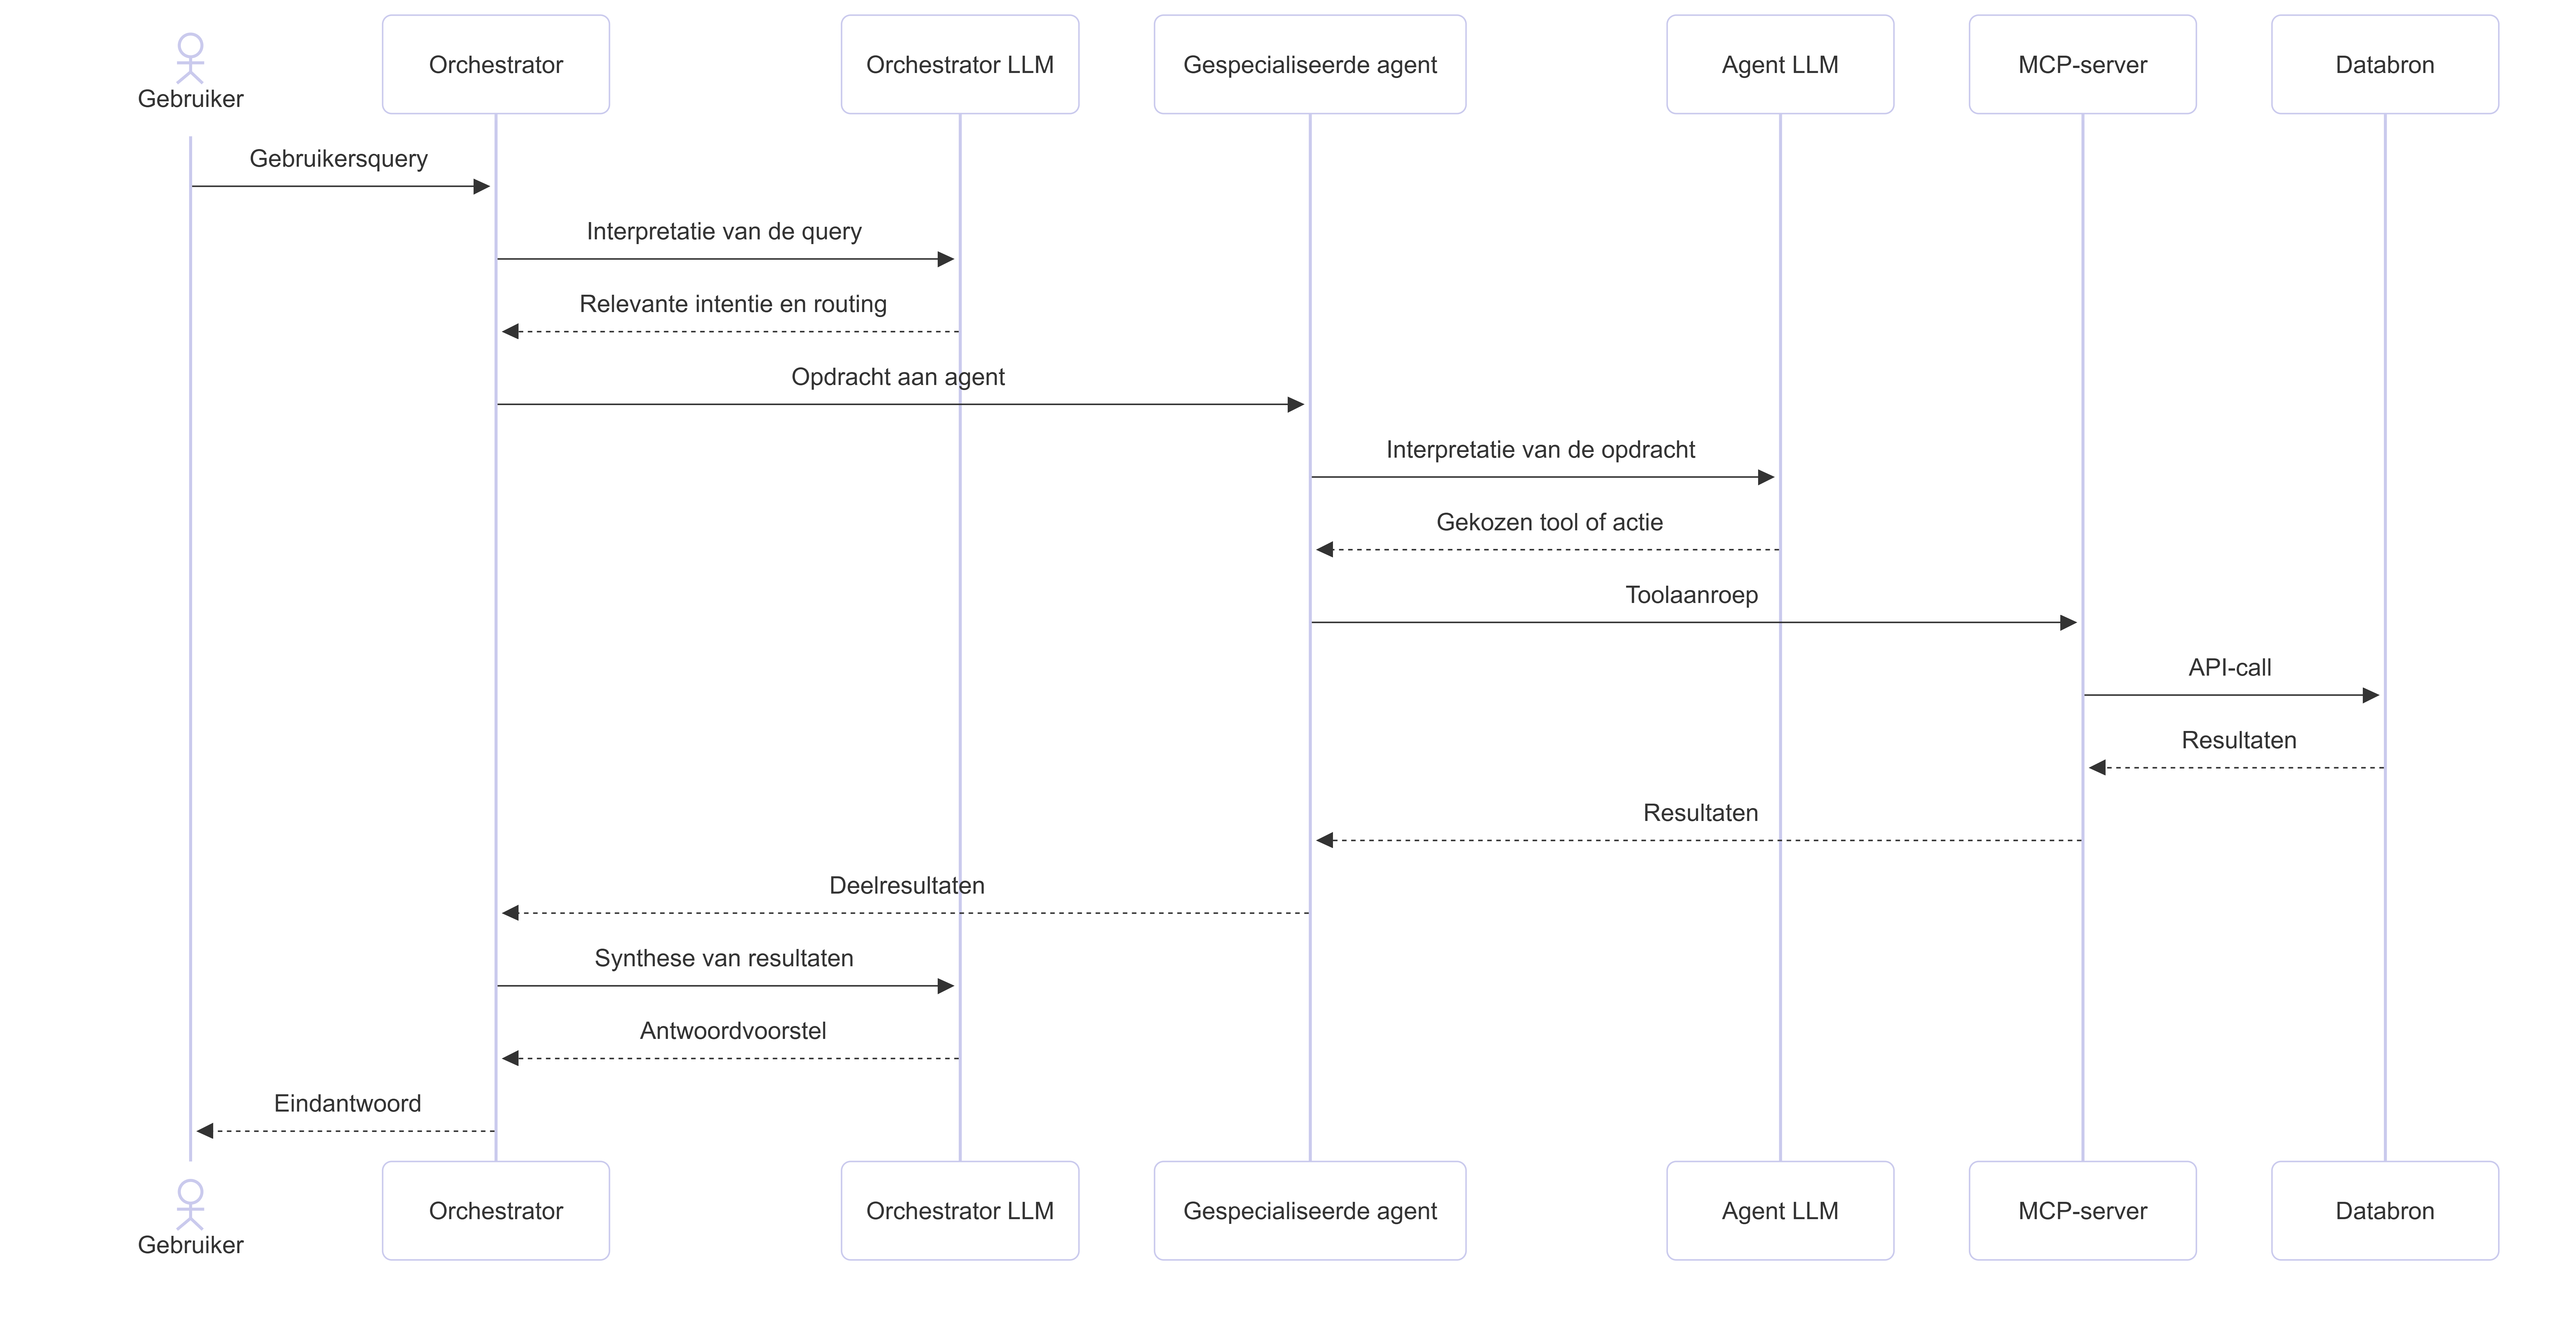
\includegraphics[width=0.80\textwidth]{verwerking_van_gebruikers_vraag}
    \caption{Schematische voorstelling van de communicatie- en queryflow: de gebruikersvraag wordt ontvangen door de orchestrator, die de relevante agents aanspreekt via de bijhorende MCP-servers. De deelresultaten worden samengevoegd tot één eindantwoord voor de gebruiker.}
    \label{fig:queryflow}
\end{figure}

\section{Veiligheids- en toegangsmodel}
\label{sec:veiligheid}

Aangezien de voorgestelde architectuur toegang biedt tot interne bedrijfsdata, vormt veiligheid een essentieel onderdeel van het ontwerp. De oplossing is daarom opgebouwd als een gecontroleerde laag bovenop bestaande bedrijfsapplicaties, waarbij de authenticatie- en autorisatiemechanismen van de onderliggende systemen behouden blijven.

Toegang tot databronnen zoals Microsoft Graph, Salesforce en SmartSales verloopt via de beveiligingsmechanismen die door deze systemen zelf worden voorzien, bijvoorbeeld via \gls{OAuth} 2.0, access tokens of andere systeemspecifieke authenticatiestromen. De architectuur verleent dus geen autonome toegang tot data, maar steunt op de rechten en toegangsmechanismen die reeds in de bronsystemen aanwezig zijn.

Een belangrijk uitgangspunt daarbij is dat de zoekoplossing geen informatie mag teruggeven waarvoor de gebruiker in het oorspronkelijke systeem geen toegangsrechten heeft. De agents en de \gls{MCP}-servers moeten deze beperkingen respecteren en mogen bestaande autorisatieregels niet omzeilen.

Daarnaast wordt de toegang tot bedrijfsdata functioneel afgebakend via gespecialiseerde agents en \gls{MCP}-tools. Het taalmodel communiceert niet rechtstreeks met de onderliggende \glspl{API}, maar kan enkel gebruikmaken van de operaties die via de voorziene agents en toollagen beschikbaar worden gesteld.



% TODO: uitwerken --- waarom gespecialiseerde subagents in plaats van de orchestrator rechtstreeks verbinden met de MCP-servers?


\section{Verantwoording van de architecturale keuzes}
\label{sec:verantwoording-keuzes}

Bij het ontwerp van de voorgestelde architectuur werd gekozen voor een multi-agentaanpak met een centrale orchestrator en gespecialiseerde subagents per databron. Die keuze is in de eerste plaats ingegeven door de heterogeniteit van de betrokken systemen. Microsoft Graph, Salesforce en SmartSales verschillen sterk in termen van APIs, authenticatie, zoekmogelijkheden en datamodellen. Door per databron een afzonderlijke agent te voorzien, blijft deze systeem-specifieke complexiteit lokaal afgebakend en wordt de architectuur beter onderhoudbaar en uitbreidbaar.

Daarnaast werd gekozen voor een centrale orchestrator om de interactie met de gebruiker te vereenvoudigen. De gebruiker moet niet zelf bepalen welke databron geraadpleegd moet worden, maar kan één vraag in natuurlijke taal formuleren. De orchestrator interpreteert deze vraag en bepaalt welke agent of combinatie van agents nodig is om tot een antwoord te komen. Op die manier wordt de routinglogica centraal georganiseerd en kunnen resultaten uit meerdere systemen samengebracht worden.

Ten slotte werd een MCP-gebaseerde integratielaag gebruikt om de agentlogica los te koppelen van de concrete systeemintegraties. Daardoor blijven de onderliggende databronnen de source of truth, terwijl de architectuur toch voldoende modulair blijft om later bijkomende databronnen of tools toe te voegen.